\synctex=1
\documentclass[11pt,aspectratio=169]{beamer}

\usepackage[T1]{fontenc}
\usepackage[french,provide=*]{babel}
\usepackage{amsmath,amssymb,amsfonts}
\usepackage{mathtools}
\usepackage{bm}
\usepackage{tikz}
\usetikzlibrary{arrows.meta,positioning,shapes,calc}
\usepackage{pgfplots}
\usepackage{xcolor}
\usepackage{booktabs}
\pgfplotsset{compat=1.18}

% Police serif pour les mathématiques
\usefonttheme[onlymath]{serif}

% Couleurs pour les figures
\definecolor{darkblue}{RGB}{0,51,102}
\definecolor{lightblue}{RGB}{230,240,250}
\definecolor{darkgreen}{RGB}{0,102,51}
\definecolor{darkred}{RGB}{153,0,0}
\definecolor{orange}{RGB}{255,128,0}
\definecolor{violet}{RGB}{102,0,153}
\definecolor{lightgreen}{RGB}{220,245,220}
\definecolor{lightorange}{RGB}{255,240,220}
\definecolor{gray}{gray}{0.4}

% Commandes mathématiques
\DeclareMathOperator*{\argmax}{arg\,max}

% Git hash
\usepackage{xstring}
\usepackage{catchfile}
\immediate\write18{git rev-parse HEAD > git.hash}
\CatchFileDef{\HEAD}{git.hash}{\endlinechar=-1}
\newcommand{\gitrevision}{\StrLeft{\HEAD}{7}}

\usepackage{ccicons}

% Pied de page personnalisé
\setbeamertemplate{footline}{
  \hfill\vspace*{1pt}\href{https://creativecommons.org/publicdomain/zero/1.0/deed.fr}{\cczero}\enspace\href{https://github.com/stepan-a/microeconometrics}{\gitrevision}\enspace--\enspace\insertframenumber/\inserttotalframenumber\enspace--\enspace\today\enspace}

% Supprimer la barre de navigation
\setbeamertemplate{navigation symbols}{}

\title{Algorithmes d'optimisation numérique}
\subtitle{Une introduction}
\author{}
\date{}
\institute{}

\AtBeginSection[]
{
  \begin{frame}
    \frametitle{Plan}
    \tableofcontents[currentsection]
  \end{frame}
}

\begin{document}

\begin{frame}
\titlepage
\end{frame}

\begin{frame}{Plan}
\tableofcontents
\end{frame}

%==============================================================================
\section{Introduction et motivation}
%==============================================================================

\begin{frame}{Introduction -- Pourquoi des algorithmes d'optimisation ?}

\begin{itemize}

\item En maximum de vraisemblance, on cherche $\hat{\theta}_N$ tel que :
  \[
  \hat{\theta}_N = \argmax_{\theta \in \Theta} \ell(y | X, \theta)
  \]
  où $\ell(\cdot)$ est la log-vraisemblance.\newline

\item En général, la condition du premier ordre :
  \[
  s(\hat{\theta}_N) = \frac{\partial \ell}{\partial \theta}\bigg|_{\hat{\theta}_N} = 0
  \]
  n'admet pas de solution analytique (contrairement aux MCO).\newline

\item $\Rightarrow$ Nécessité de méthodes \textbf{numériques itératives}.

\end{itemize}

\end{frame}

\begin{frame}{Introduction -- Notations}

\begin{itemize}

\item $\ell(\theta)$ : log-vraisemblance (fonction à maximiser)\newline

\item $s(\theta) = \dfrac{\partial \ell(\theta)}{\partial \theta}$ : \textbf{score} (gradient, vecteur $p \times 1$)\newline

\item $H(\theta) = \dfrac{\partial^2 \ell(\theta)}{\partial \theta \partial \theta'}$ : \textbf{hessien} (matrice $p \times p$)\newline

\item Contributions individuelles :
  \[
  \ell(\theta) = \sum_{i=1}^{N} \ln f(y_i | X_i, \theta), \quad s(\theta) = \sum_{i=1}^{N} \frac{\partial \ln f_i}{\partial \theta}, \quad H(\theta) = \sum_{i=1}^{N} \frac{\partial^2 \ln f_i}{\partial \theta \partial \theta'}
  \]

\end{itemize}

\end{frame}

\begin{frame}{Introduction -- Concavité et unicité}

\begin{itemize}

\item $\ell(\theta)$ est \textbf{concave} si $H(\theta) \prec 0$ (définie négative) pour tout $\theta \in \Theta$.\newline

\item Conséquences de la concavité :
  \begin{itemize}
    \item Le maximum est unique\newline
    \item La CPO $s(\hat{\theta}_N) = 0$ est suffisante\newline
    \item Tout algorithme croissant converge vers ce maximum\newline
  \end{itemize}

\item Modèles à log-vraisemblance concave : \textbf{Logit}, \textbf{Probit}, \textbf{Poisson}, modèle linéaire gaussien.

\end{itemize}

\end{frame}

\begin{frame}{Introduction -- Concavité (illustration)}

\begin{center}
    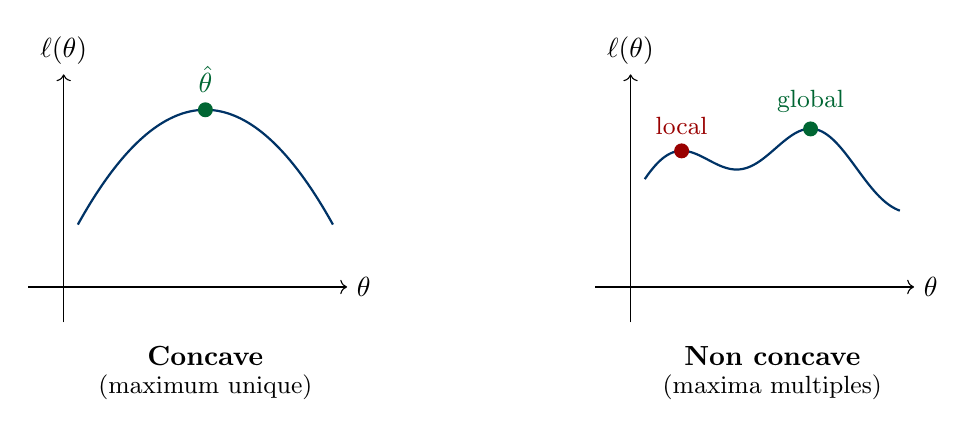
\begin{tikzpicture}[scale=0.9]
        % Fonction concave
        \begin{scope}[shift={(-4,0)}]
            \draw[->] (-0.5,0) -- (4,0) node[right] {$\theta$};
            \draw[->] (0,-0.5) -- (0,3) node[above] {$\ell(\theta)$};
            \draw[thick, darkblue, domain=0.2:3.8, samples=100] plot (\x, {-0.5*(\x-2)^2 + 2.5});
            \fill[darkgreen] (2,2.5) circle (3pt);
            \node[above, darkgreen] at (2,2.6) {$\hat{\theta}$};
            \node[below] at (2,-0.7) {\textbf{Concave}};
            \node[below, font=\small] at (2,-1.1) {(maximum unique)};
        \end{scope}
        % Fonction non concave
        \begin{scope}[shift={(4,0)}]
            \draw[->] (-0.5,0) -- (4,0) node[right] {$\theta$};
            \draw[->] (0,-0.5) -- (0,3) node[above] {$\ell(\theta)$};
            \draw[thick, darkblue, domain=0.2:3.8, samples=100] plot (\x, {0.3*sin(3*\x r) - 0.2*(\x-2)^2 + 2});
            \fill[darkred] (0.72,1.92) circle (3pt);
            \fill[darkgreen] (2.54,2.23) circle (3pt);
            \node[above, darkred, font=\small] at (0.72,2.02) {local};
            \node[above, darkgreen, font=\small] at (2.54,2.33) {global};
            \node[below] at (2,-0.7) {\textbf{Non concave}};
            \node[below, font=\small] at (2,-1.1) {(maxima multiples)};
        \end{scope}
    \end{tikzpicture}
\end{center}

\end{frame}

%==============================================================================
\section{Structure générale d'un algorithme}
%==============================================================================

\begin{frame}{Algorithme -- Les quatre composantes}

\begin{enumerate}
    \item \textbf{Valeur initiale} $\theta_{(0)}$\newline
    \item \textbf{Règle d'itération} : $\theta_{(p+1)} = \theta_{(p)} + M(\theta_{(p)})$\newline
    \item \textbf{Critère d'arrêt} : quand s'arrêter ?\newline
    \item \textbf{Vérification} : a-t-on bien un maximum ?
\end{enumerate}

\vspace{0.3cm}

\begin{center}
    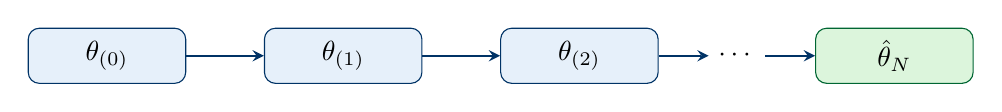
\begin{tikzpicture}[
        box/.style={rectangle, draw=darkblue, fill=lightblue, minimum width=2cm, minimum height=0.7cm, rounded corners},
        arrow/.style={->, >=stealth, thick, darkblue}
    ]
    \node[box] (a) at (0,0) {$\theta_{(0)}$};
    \node[box] (b) at (3,0) {$\theta_{(1)}$};
    \node[box] (c) at (6,0) {$\theta_{(2)}$};
    \node (d) at (8,0) {$\cdots$};
    \node[box, fill=lightgreen, draw=darkgreen] (e) at (10,0) {$\hat{\theta}_N$};
    \draw[arrow] (a) -- (b);
    \draw[arrow] (b) -- (c);
    \draw[arrow] (c) -- (d);
    \draw[arrow] (d) -- (e);
    \end{tikzpicture}
\end{center}

\end{frame}

\begin{frame}{Algorithme -- Choix de la valeur initiale}

\begin{itemize}

\item \textbf{Cas d'une fonction concave :}
  \begin{itemize}
    \item Tout point de départ mène au maximum (avec un algorithme croissant)\newline
    \item On peut prendre $\theta_{(0)} = 0$ ou une valeur raisonnable\newline
  \end{itemize}

\item \textbf{Cas d'une fonction non concave :}
  \begin{itemize}
    \item Le choix de $\theta_{(0)}$ est crucial\newline
    \item Utiliser un estimateur convergent comme point de départ\newline
    \item Exemple : estimateur en deux étapes (plus simple mais inefficace)\newline
  \end{itemize}

\item Un bon point de départ accélère la convergence, même avec une fonction concave.

\end{itemize}

\end{frame}

\begin{frame}{Algorithme -- Règle d'itération}

\begin{itemize}

\item Forme générale :
  \[
  \theta_{(p+1)} = \theta_{(p)} + M(\theta_{(p)})
  \]
  où $M(\theta_{(p)})$ est le \textbf{pas de l'itération}.\newline

\item Propriétés souhaitables :
  \begin{itemize}
    \item Le pas ne dépend que de $\theta_{(p)}$ (et des données)\newline
    \item À l'optimum : $M(\hat{\theta}_N) = 0$ (stationnarité)\newline
    \item L'algorithme est \textbf{croissant} : $\ell(\theta_{(p+1)}) \geq \ell(\theta_{(p)})$\newline
  \end{itemize}

\item Les différents algorithmes diffèrent par leur définition de $M(\cdot)$.

\end{itemize}

\end{frame}

\begin{frame}{Algorithme -- Critères d'arrêt}

\begin{enumerate}

\item \textbf{Variation de l'objectif :} $|\ell(\theta_{(p+1)}) - \ell(\theta_{(p)})| < \varepsilon_1$\newline

\item \textbf{Norme du gradient :} $\|s(\theta_{(p)})\| < \varepsilon_2$\newline

\item \textbf{Variation des paramètres :} $\|\theta_{(p+1)} - \theta_{(p)}\| < \varepsilon_3$\newline

\item \textbf{Élasticité} (insensible aux unités) : $\left|\frac{\theta_{(p)}}{\ell(\theta_{(p)})} \cdot s(\theta_{(p)})\right| < \varepsilon_4$

\end{enumerate}

\vspace{0.3cm}

À l'optimum, tous ces critères sont équivalents (tous nuls).

\end{frame}

\begin{frame}{Algorithme -- Vérification du maximum}

\begin{itemize}

\item Pour un \textbf{maximum local}, le hessien doit être défini négatif :
  \[
  H(\hat{\theta}_N) = \frac{\partial^2 \ell}{\partial \theta \partial \theta'}\bigg|_{\hat{\theta}_N} \prec 0
  \]

\item Importance pratique :
  \begin{itemize}
    \item Si $H(\hat{\theta}_N) \not\prec 0$ : on n'est pas à un maximum !\newline
    \item L'inverse du hessien estime la variance : $\widehat{\mathrm{Var}}(\hat{\theta}_N) \approx -H(\hat{\theta}_N)^{-1}$\newline
    \item Si $H$ n'est pas définie négative $\Rightarrow$ variance non définie positive $\Rightarrow$ inutilisable
  \end{itemize}

\end{itemize}

\end{frame}

\begin{frame}{Algorithme -- Schéma complet}

\begin{center}
    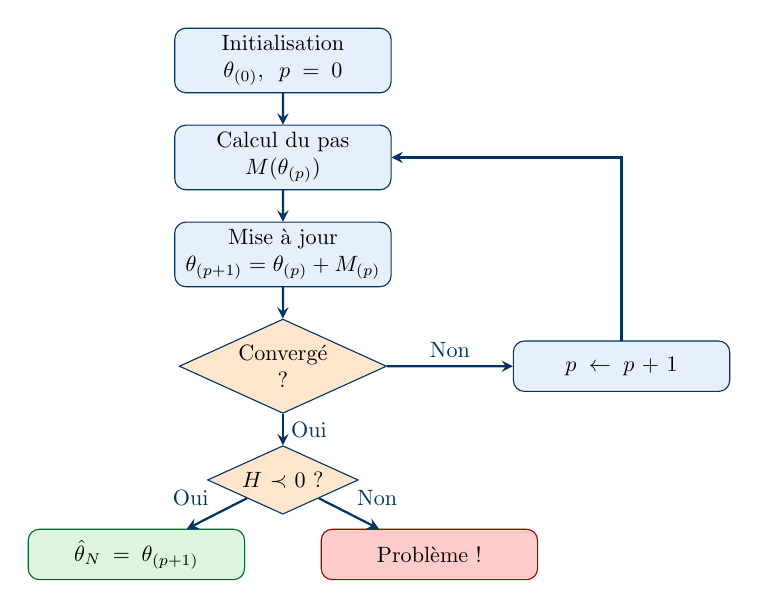
\begin{tikzpicture}[scale=0.8, every node/.style={transform shape},
        node distance=0.7cm,
        box/.style={rectangle, draw=darkblue, fill=lightblue, text width=3.2cm, align=center, minimum height=0.8cm, rounded corners},
        decision/.style={diamond, draw=darkblue, fill=orange!20, text width=1.6cm, align=center, aspect=2.2, inner sep=1pt},
        arrow/.style={->, >=stealth, thick, darkblue}
    ]
    \node[box] (init) {Initialisation\\$\theta_{(0)}, \; p = 0$};
    \node[box, below=0.5cm of init] (iter) {Calcul du pas\\$M(\theta_{(p)})$};
    \node[box, below=0.5cm of iter] (update) {Mise à jour\\$\theta_{(p+1)} = \theta_{(p)} + M_{(p)}$};
    \node[decision, below=0.5cm of update] (conv) {Convergé ?};
    \node[box, right=2cm of conv] (incr) {$p \leftarrow p+1$};
    \node[decision, below=0.5cm of conv] (cso) {$H \prec 0$ ?};
    \node[box, below left=0.5cm and 0cm of cso, fill=lightgreen, draw=darkgreen] (ok) {$\hat{\theta}_N = \theta_{(p+1)}$};
    \node[box, below right=0.5cm and 0cm of cso, fill=red!20, draw=darkred] (nok) {Problème !};
    \draw[arrow] (init) -- (iter);
    \draw[arrow] (iter) -- (update);
    \draw[arrow] (update) -- (conv);
    \draw[arrow] (conv) -- node[above] {Non} (incr);
    \draw[arrow] (incr) |- (iter);
    \draw[arrow] (conv) -- node[right] {Oui} (cso);
    \draw[arrow] (cso) -- node[above left] {Oui} (ok);
    \draw[arrow] (cso) -- node[above right] {Non} (nok);
    \end{tikzpicture}
\end{center}

\end{frame}

%==============================================================================
\section{Les méthodes de gradient}
%==============================================================================

\begin{frame}{Gradient -- Principe général}

\begin{itemize}

\item Un algorithme de gradient suit la règle d'itération :
  \[
  \boxed{\theta_{(p+1)} = \theta_{(p)} + \lambda W_{(p)} s(\theta_{(p)})}
  \]
  où :
  \begin{itemize}
    \item $s(\theta_{(p)})$ : gradient (score) au point courant\newline
    \item $W_{(p)}$ : matrice de pondération ($p \times p$, symétrique)\newline
    \item $\lambda \in (0, 1]$ : paramètre de pas (\textit{step size})\newline
  \end{itemize}

\item À l'optimum : $s(\hat{\theta}_N) = 0$ donc le pas est nul et l'algorithme s'arrête.

\end{itemize}

\end{frame}

\begin{frame}{Gradient -- Le paramètre de pas $\lambda$}

\begin{itemize}

\item Contrôle l'amplitude du déplacement. Par défaut : $\lambda = 1$.\newline

\item Si $\ell(\theta_{(p+1)}) < \ell(\theta_{(p)})$ : réduire $\lambda$ (\textit{line search}).

\end{itemize}

\vspace{0.3cm}

\begin{center}
    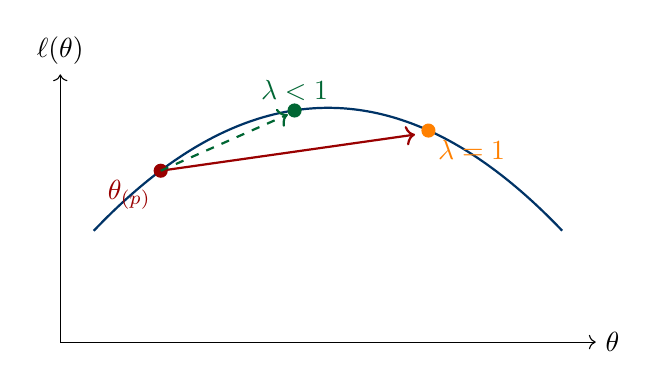
\begin{tikzpicture}[scale=0.85]
        \draw[->] (0,0) -- (8,0) node[right] {$\theta$};
        \draw[->] (0,0) -- (0,4) node[above] {$\ell(\theta)$};
        \draw[thick, darkblue, domain=0.5:7.5, samples=100] plot (\x, {-0.15*(\x-4)^2 + 3.5});
        \fill[darkred] (1.5,2.56) circle (3pt) node[below left] {$\theta_{(p)}$};
        \fill[orange] (5.5,3.16) circle (3pt) node[below right] {$\lambda = 1$};
        \fill[darkgreen] (3.5,3.46) circle (3pt) node[above] {$\lambda < 1$};
        \draw[->, thick, darkred] (1.5,2.56) -- (5.3,3.1);
        \draw[->, thick, dashed, darkgreen] (1.5,2.56) -- (3.4,3.4);
    \end{tikzpicture}
\end{center}

\end{frame}

\begin{frame}{Gradient -- Propriété de croissance}

\begin{alertblock}{Théorème}
Si $W_{(p)}$ est symétrique définie positive, alors pour $\lambda$ suffisamment petit :
\[
\ell(\theta_{(p+1)}) \geq \ell(\theta_{(p)})
\]
\end{alertblock}

\begin{itemize}

\item Idée de la preuve. Développement de Taylor :
  \[
  \ell(\theta_{(p+1)}) \approx \ell(\theta_{(p)}) + \lambda \underbrace{s(\theta_{(p)})' W_{(p)} s(\theta_{(p)})}_{> 0 \text{ si } W_{(p)} \succ 0}
  \]

\item Pour une fonction concave, un algorithme croissant converge vers le maximum global.

\end{itemize}

\end{frame}

\begin{frame}{Gradient -- Vue d'ensemble}

\begin{center}
    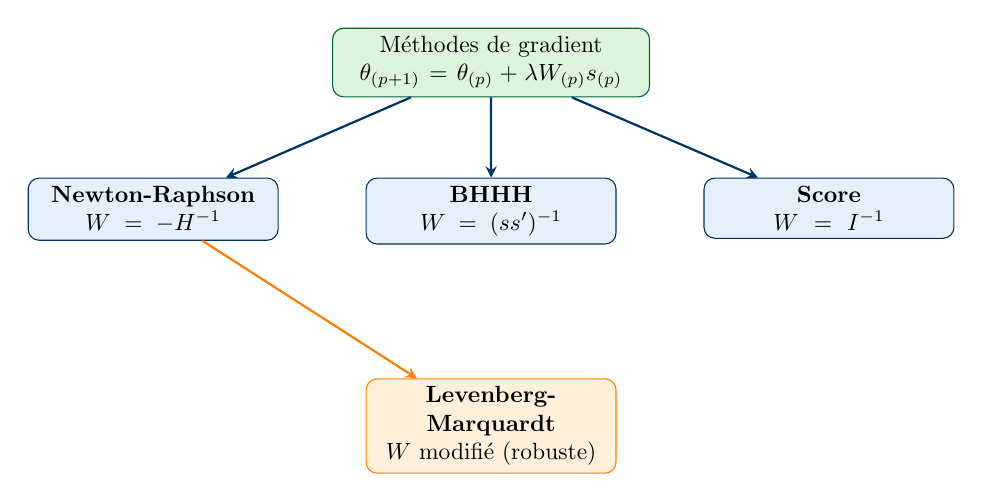
\begin{tikzpicture}[scale=0.85, every node/.style={transform shape},
        node distance=1cm,
        mainbox/.style={rectangle, draw=darkgreen, fill=lightgreen, text width=4.5cm, align=center, minimum height=1cm, rounded corners},
        box/.style={rectangle, draw=darkblue, fill=lightblue, text width=3.5cm, align=center, minimum height=0.9cm, rounded corners},
        arrow/.style={->, >=stealth, thick, darkblue}
    ]
    \node[mainbox] (grad) {Méthodes de gradient\\$\theta_{(p+1)} = \theta_{(p)} + \lambda W_{(p)} s_{(p)}$};
    \node[box, below left=1.2cm and 0.8cm of grad] (nr) {\textbf{Newton-Raphson}\\$W = -H^{-1}$};
    \node[box, below=1.2cm of grad] (bhhh) {\textbf{BHHH}\\$W = (ss')^{-1}$};
    \node[box, below right=1.2cm and 0.8cm of grad] (score) {\textbf{Score}\\$W = I^{-1}$};
    \draw[arrow] (grad) -- (nr);
    \draw[arrow] (grad) -- (bhhh);
    \draw[arrow] (grad) -- (score);
    \node[box, below=2cm of bhhh, fill=lightorange, draw=orange] (lm) {\textbf{Levenberg-Marquardt}\\$W$ modifié (robuste)};
    \draw[arrow, orange] (nr) -- (lm);
    \end{tikzpicture}
\end{center}

\end{frame}

%==============================================================================
\section{Algorithme de Newton-Raphson}
%==============================================================================

\begin{frame}{Newton-Raphson -- Principe}

\begin{itemize}

\item \textbf{Idée :} Approximer $\ell(\theta)$ par une fonction quadratique au voisinage de $\theta_{(p)}$, puis maximiser cette approximation.\newline

\item Développement de Taylor (ordre 2) :
  \[
  \ell(\theta) \approx \ell(\theta_{(p)}) + s(\theta_{(p)})'(\theta - \theta_{(p)}) + \frac{1}{2}(\theta - \theta_{(p)})'H(\theta_{(p)})(\theta - \theta_{(p)})
  \]

\end{itemize}

\vspace{0.2cm}

\begin{center}
    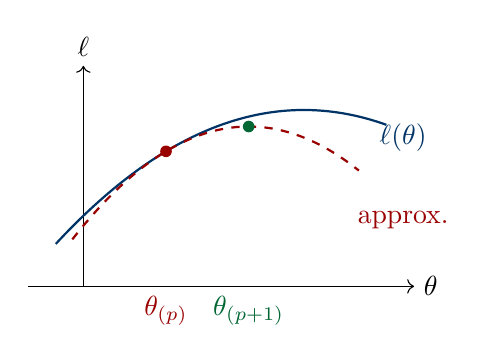
\begin{tikzpicture}[scale=0.7]
        \draw[->] (-1,0) -- (6,0) node[right] {$\theta$};
        \draw[->] (0,0) -- (0,4) node[above] {$\ell$};
        \draw[thick, darkblue, domain=-0.5:5.5, samples=100] plot (\x, {-0.12*(\x-4)^2 + 3.2});
        \draw[thick, dashed, darkred, domain=-0.2:5, samples=50] plot (\x, {-0.2*(\x-3)^2 + 2.9});
        \fill[darkred] (1.5,2.45) circle (3pt);
        \fill[darkgreen] (3,2.9) circle (3pt);
        \node[below, darkred] at (1.5,0) {$\theta_{(p)}$};
        \node[below, darkgreen] at (3,0) {$\theta_{(p+1)}$};
        \node[right, darkred] at (4.8,1.2) {approx.};
        \node[right, darkblue] at (5.2,2.7) {$\ell(\theta)$};
    \end{tikzpicture}
\end{center}

\end{frame}

\begin{frame}{Newton-Raphson -- Dérivation}

\begin{itemize}

\item Maximisation de l'approximation quadratique (CPO) :
  \[
  s(\theta_{(p)}) + H(\theta_{(p)})(\theta - \theta_{(p)}) = 0
  \]

\item Solution :
  \[
  \theta - \theta_{(p)} = -H(\theta_{(p)})^{-1} s(\theta_{(p)})
  \]

\item Règle d'itération :
  \[
  \boxed{\theta_{(p+1)} = \theta_{(p)} - \lambda H(\theta_{(p)})^{-1} s(\theta_{(p)})}
  \]
  Ici : $W_{(p)} = -H(\theta_{(p)})^{-1}$

\end{itemize}

\end{frame}

\begin{frame}{Newton-Raphson -- Propriétés}

\begin{itemize}

\item \textbf{Avantages :}
  \begin{itemize}
    \item Convergence rapide (quadratique près de l'optimum)\newline
    \item Peu d'itérations en général\newline
    \item Vérifie la CSO (on calcule $H$ à chaque itération)\newline
    \item Fournit la variance : $\widehat{\mathrm{Var}}(\hat{\theta}_N) \approx -H(\hat{\theta}_N)^{-1}$\newline
  \end{itemize}

\item \textbf{Inconvénients :}
  \begin{itemize}
    \item Nécessite le calcul des dérivées secondes\newline
    \item Coûteux en temps si dérivées numériques\newline
    \item Peut diverger si $H$ n'est pas définie négative\newline
    \item Sensible au point de départ si fonction non concave
  \end{itemize}

\end{itemize}

\end{frame}

\begin{frame}{Newton-Raphson -- Convergence}

\begin{center}
    \begin{tikzpicture}[scale=1]
        \draw[->] (0,0) -- (9,0) node[right] {$\theta$};
        \draw[->] (0,0) -- (0,4.5) node[above] {$\ell(\theta)$};
        \draw[thick, darkblue, domain=0.5:8.5, samples=100] plot (\x, {-0.08*(\x-5)^2 + 4});
        \fill[darkred] (1.5,3.02) circle (3pt);
        \node[below, darkred] at (1.5,0) {$\theta_{(0)}$};
        \fill[orange] (3.8,3.88) circle (3pt);
        \node[below, orange] at (3.8,0) {$\theta_{(1)}$};
        \fill[darkgreen] (4.85,4.0) circle (3pt);
        \node[below, darkgreen] at (4.85,0) {$\theta_{(2)}$};
        \fill[violet] (5,4) circle (3pt);
        \node[above, violet] at (5,4.1) {$\hat{\theta}$};
        \draw[->, thick, darkred] (1.5,3.02) to[bend left=15] (3.7,3.85);
        \draw[->, thick, orange] (3.8,3.88) to[bend left=10] (4.8,3.98);
    \end{tikzpicture}
\end{center}

\vspace{0.3cm}

Newton-Raphson converge souvent en \textbf{3 à 5 itérations} pour des problèmes bien conditionnés.

\end{frame}

%==============================================================================
\section{Algorithme BHHH}
%==============================================================================

\begin{frame}{BHHH -- Motivation}

\begin{itemize}

\item Le calcul du hessien $H(\theta)$ peut être complexe analytiquement ou coûteux numériquement.\newline

\item \textbf{Idée :} Utiliser l'égalité de la matrice d'information :
  \[
  \mathbb{E}\left[-\frac{\partial^2 \ln f}{\partial \theta \partial \theta'}\right] = \mathbb{E}\left[\frac{\partial \ln f}{\partial \theta}\frac{\partial \ln f}{\partial \theta'}\right]
  \]

\item $\Rightarrow$ Approximer $-H(\theta)$ par les \textbf{produits croisés du score}.

\end{itemize}

\end{frame}

\begin{frame}{BHHH -- Approximation du hessien}

\begin{itemize}

\item On remplace :
  \[
  -H(\theta) = -\sum_{i=1}^{N}\frac{\partial^2 \ln f_i}{\partial \theta \partial \theta'}
  \]
  par :
  \[
  \sum_{i=1}^{N}\frac{\partial \ln f_i}{\partial \theta}\frac{\partial \ln f_i}{\partial \theta'} = \sum_{i=1}^{N} s_i s_i'
  \]
  où $s_i = \frac{\partial \ln f_i}{\partial \theta}$ est le score individuel.\newline

\item Cette matrice est automatiquement semi-définie positive (somme de matrices $s_i s_i' \succeq 0$).

\end{itemize}

\end{frame}

\begin{frame}{BHHH -- Règle d'itération}

\begin{itemize}

\item Règle d'itération :
  \[
  \boxed{\theta_{(p+1)} = \theta_{(p)} + \lambda \left(\sum_{i=1}^{N} s_i(\theta_{(p)}) s_i(\theta_{(p)})'\right)^{-1} s(\theta_{(p)})}
  \]
  où $s_i(\theta) = \frac{\partial \ln f(y_i | X_i, \theta)}{\partial \theta}$ et $s(\theta) = \sum_i s_i(\theta)$.\newline

\item En notation compacte, soit $S$ la matrice $N \times p$ des scores individuels (ligne $i$ : $s_i'$) :
  \[
  W_{(p)} = (S'S)^{-1}
  \]

\end{itemize}

\end{frame}

\begin{frame}{BHHH -- Propriétés}

\begin{itemize}

\item \textbf{Avantages :}
  \begin{itemize}
    \item Ne nécessite que les dérivées premières\newline
    \item Facile à programmer\newline
    \item $W_{(p)} = (S'S)^{-1}$ est toujours définie positive\newline
    \item Algorithme toujours croissant\newline
  \end{itemize}

\item \textbf{Inconvénients :}
  \begin{itemize}
    \item Convergence plus lente que Newton-Raphson\newline
    \item Plus d'itérations nécessaires\newline
    \item Ne vérifie pas directement que $H \prec 0$\newline
    \item L'approximation peut être mauvaise loin de l'optimum
  \end{itemize}

\end{itemize}

\end{frame}

\begin{frame}{BHHH -- Convergence}

\begin{center}
    \begin{tikzpicture}[scale=1]
        \draw[->] (0,0) -- (9,0) node[right] {$\theta$};
        \draw[->] (0,0) -- (0,4.5) node[above] {$\ell(\theta)$};
        \draw[thick, darkblue, domain=0.5:8.5, samples=100] plot (\x, {-0.08*(\x-5)^2 + 4});
        \fill[darkred] (1.5,3.02) circle (2.5pt);
        \fill[orange] (2.8,3.61) circle (2.5pt);
        \fill[yellow!70!orange] (3.7,3.86) circle (2.5pt);
        \fill[green!70!yellow] (4.3,3.96) circle (2.5pt);
        \fill[darkgreen] (4.7,3.99) circle (2.5pt);
        \fill[violet] (5,4) circle (3pt);
        \node[below, darkred] at (1.5,0) {$\theta_{(0)}$};
        \node[above, violet] at (5,4.1) {$\hat{\theta}$};
        \draw[dashed, gray] (1.5,3.02) -- (2.8,3.61) -- (3.7,3.86) -- (4.3,3.96) -- (4.7,3.99) -- (5,4);
    \end{tikzpicture}
\end{center}

\vspace{0.3cm}

BHHH fait des \textbf{pas plus petits} que Newton-Raphson $\Rightarrow$ plus d'itérations mais plus stable.

\end{frame}

%==============================================================================
\section{Algorithme du Score}
%==============================================================================

\begin{frame}{Score -- Principe}

\begin{itemize}

\item \textbf{Idée :} Raffinement de BHHH. Remplacer les produits croisés du score par leur espérance mathématique (information de Fisher).\newline

\item Approximation :
  \[
  -H(\theta) \approx \sum_{i=1}^{N} \mathbb{E}_y\left[\frac{\partial \ln f_i}{\partial \theta}\frac{\partial \ln f_i}{\partial \theta'}\right] = N \cdot I_1(\theta)
  \]
  où $I_1(\theta)$ est l'information de Fisher pour une observation.

\end{itemize}

\end{frame}

\begin{frame}{Score -- Règle d'itération}

\begin{itemize}

\item Règle d'itération :
  \[
  \boxed{\theta_{(p+1)} = \theta_{(p)} + \lambda \left(\sum_{i=1}^{N} \mathbb{E}_y\left[s_i s_i'\right]\bigg|_{\theta_{(p)}}\right)^{-1} s(\theta_{(p)})}
  \]

\item Simplification :
  \[
  W_{(p)} = I_N(\theta_{(p)})^{-1} = \frac{1}{N} I_1(\theta_{(p)})^{-1}
  \]

\item L'algorithme du Score utilise l'information de Fisher \textbf{théorique} plutôt qu'empirique.

\end{itemize}

\end{frame}

\begin{frame}{Score -- Équivalence avec Newton-Raphson}

\begin{alertblock}{Théorème}
Si les dérivées secondes de $\ln f$ ne dépendent pas de $y$, alors :
\[
\mathbb{E}_y\left[-\frac{\partial^2 \ln f}{\partial \theta \partial \theta'}\right] = -\frac{\partial^2 \ln f}{\partial \theta \partial \theta'}
\]
et l'algorithme du Score est \textbf{identique} à Newton-Raphson.
\end{alertblock}

\begin{itemize}

\item Modèles où Score = Newton-Raphson :
  \begin{itemize}
    \item \textbf{Logit} : $H$ ne dépend que de $X$ et $\theta$\newline
    \item \textbf{Poisson} : idem\newline
    \item Modèle linéaire gaussien
  \end{itemize}

\end{itemize}

\end{frame}

%==============================================================================
\section{Algorithme de Levenberg-Marquardt}
%==============================================================================

\begin{frame}{Levenberg-Marquardt -- Problème de départ}

\begin{itemize}

\item Si $H(\theta_{(p)})$ n'est pas définie négative au point $\theta_{(p)}$ :
  \begin{itemize}
    \item Newton-Raphson n'est plus garanti croissant\newline
    \item L'algorithme peut diverger\newline
    \item BHHH peut avoir une valeur propre nulle $\Rightarrow$ non inversible\newline
  \end{itemize}

\end{itemize}

\begin{center}
    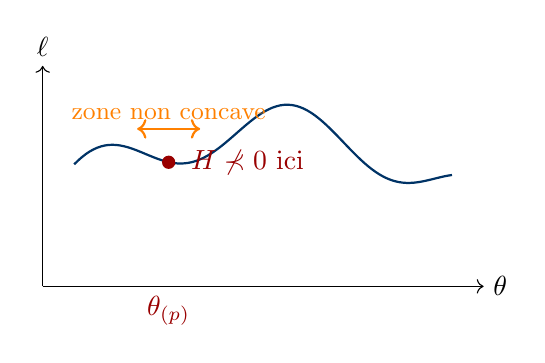
\begin{tikzpicture}[scale=0.8]
        \draw[->] (0,0) -- (7,0) node[right] {$\theta$};
        \draw[->] (0,0) -- (0,3.5) node[above] {$\ell$};
        \draw[thick, darkblue, domain=0.5:6.5, samples=100] plot (\x, {0.4*sin(2*\x r) - 0.1*(\x-3.5)^2 + 2.5});
        \fill[darkred] (2,1.97) circle (3pt);
        \node[below, darkred] at (2,0) {$\theta_{(p)}$};
        \node[right, darkred] at (2.2,1.97) {$H \not\prec 0$ ici};
        \draw[<->, thick, orange] (1.5,2.5) -- (2.5,2.5);
        \node[above, orange, font=\small] at (2,2.5) {zone non concave};
    \end{tikzpicture}
\end{center}

\end{frame}

\begin{frame}{Levenberg-Marquardt -- Idée}

\begin{itemize}

\item \textbf{Solution :} Modifier le hessien pour le rendre défini négatif, tout en restant aussi proche que possible de l'original.\newline

\item On remplace $H(\theta_{(p)})$ par :
  \[
  \boxed{\tilde{H}_{(p)} = H(\theta_{(p)}) - (1 + \alpha)\mu_H I_k}
  \]
  où :
  \begin{itemize}
    \item $\mu_H$ : plus grande valeur propre de $H(\theta_{(p)})$ (supposée $> 0$)\newline
    \item $\alpha > 0$ : paramètre choisi par l'utilisateur (petit)\newline
    \item $I_k$ : matrice identité de dimension $k$ (taille de $\theta$)
  \end{itemize}

\end{itemize}

\end{frame}

\begin{frame}{Levenberg-Marquardt -- Justification}

\begin{itemize}

\item Si $\lambda_1, \ldots, \lambda_k$ sont les valeurs propres de $H$, alors les valeurs propres de $\tilde{H}$ sont :
  \[
  \tilde{\lambda}_j = \lambda_j - (1+\alpha)\mu_H
  \]

\item En particulier, pour $\lambda_j = \mu_H$ (la plus grande) :
  \[
  \tilde{\lambda}_j = \mu_H - (1+\alpha)\mu_H = -\alpha \mu_H < 0
  \]

\item Toutes les valeurs propres de $\tilde{H}$ sont strictement négatives $\Rightarrow$ $\tilde{H} \prec 0$.

\end{itemize}

\end{frame}

\begin{frame}{Levenberg-Marquardt -- Règle d'itération}

\begin{itemize}

\item Règle complète :
  \[
  \theta_{(p+1)} = \begin{cases}
      \theta_{(p)} - \lambda \left(H(\theta_{(p)}) - (1+\alpha)\mu_H I_k\right)^{-1} s(\theta_{(p)}) & \text{si } \mu_H \geq 0 \\[0.3cm]
      \theta_{(p)} - \lambda H(\theta_{(p)})^{-1} s(\theta_{(p)}) & \text{si } \mu_H < 0
  \end{cases}
  \]

\item Si $\mu_H < 0$ : $H \prec 0$ donc on utilise Newton-Raphson standard.\newline

\item Si $\mu_H \geq 0$ : on modifie $H$ pour le rendre défini négatif.

\end{itemize}

\end{frame}

\begin{frame}{Levenberg-Marquardt -- Choix de $\alpha$}

\begin{itemize}

\item Commencer avec une petite valeur : $\alpha = 0.01$ ou $0.1$.\newline

\item Observer l'évolution de $\mu_H$ au fil des itérations :
  \begin{itemize}
    \item Si $\mu_H$ croît : $\alpha$ trop élevé\newline
    \item Si $\mu_H$ tend vers 0 : $\alpha$ trop petit\newline
    \item Valeur correcte : comportement intermédiaire\newline
  \end{itemize}

\item L'algorithme peut être sensible à de petites variations de $\alpha$ (ex. : $\alpha = 0.1$ fonctionne, $\alpha = 0.2$ diverge).\newline

\item Une fois $\alpha$ trouvé pour un échantillon, on le garde généralement constant.

\end{itemize}

\end{frame}

\begin{frame}{Levenberg-Marquardt -- Applications}

\begin{itemize}

\item \textbf{Modèles à objectif non concave :}
  \begin{itemize}
    \item Tobit généralisé (modèle de Heckman)\newline
    \item Moindres carrés non linéaires\newline
    \item Modèles à équations simultanées\newline
    \item Certains modèles de mélange\newline
  \end{itemize}

\item \textbf{Avantages :}
  \begin{itemize}
    \item Robuste : fonctionne même si $H$ n'est pas définie négative\newline
    \item Retrouve Newton-Raphson dans les zones concaves\newline
    \item Permet de traverser les régions non concaves
  \end{itemize}

\end{itemize}

\end{frame}

%==============================================================================
\section{Comparaison et recommandations}
%==============================================================================

\begin{frame}{Comparaison -- Tableau récapitulatif}

\begin{center}
    \small
    \renewcommand{\arraystretch}{1.3}
    \begin{tabular}{lcccc}
        \toprule
        \textbf{Algorithme} & \textbf{Matrice $W$} & \textbf{Dérivées} & \textbf{Vitesse} & \textbf{Robustesse} \\
        \midrule
        Newton-Raphson & $-H^{-1}$ & 2nd ordre & $\star\star\star$ & $\star$ \\
        BHHH & $(SS')^{-1}$ & 1er ordre & $\star$ & $\star\star$ \\
        Score & $I^{-1}$ & $\mathbb{E}[ss']$ & $\star\star$ & $\star\star$ \\
        Levenberg-Marquardt & $-\tilde{H}^{-1}$ & 2nd ordre & $\star\star$ & $\star\star\star$ \\
        \bottomrule
    \end{tabular}
\end{center}

\vspace{0.5cm}

$\star$ = faible, $\star\star$ = moyen, $\star\star\star$ = élevé

\end{frame}

\begin{frame}{Comparaison -- Guide de choix}

\begin{itemize}

\item \textbf{Fonction objectif concave (cas usuel) :}
  \begin{enumerate}
    \item Newton-Raphson si dérivées analytiques disponibles\newline
    \item BHHH pour le prototypage ou si dérivées 2nd ordre complexes\newline
    \item Score si $H$ ne dépend pas de $y$ (équivalent à N-R)\newline
  \end{enumerate}

\item \textbf{Fonction objectif non concave :}
  \begin{enumerate}
    \item Levenberg-Marquardt : choix par défaut\newline
    \item Commencer par un bon point initial (estimateur convergent)\newline
    \item Ajuster $\alpha$ si nécessaire
  \end{enumerate}

\end{itemize}

\end{frame}

\begin{frame}{Comparaison -- Stratégie pratique}

\begin{enumerate}

\item \textbf{Phase de développement :}
  \begin{itemize}
    \item Utiliser BHHH (plus simple à coder)
    \item Vérifier numériquement les dérivées premières
  \end{itemize}

  \vspace{0.3cm}

\item \textbf{Phase de production :}
  \begin{itemize}
    \item Passer à Newton-Raphson pour la vitesse
    \item Vérifier numériquement les dérivées secondes
  \end{itemize}

  \vspace{0.3cm}

\item \textbf{En cas de problème :}
  \begin{itemize}
    \item Utiliser Levenberg-Marquardt
    \item Vérifier le point de départ
    \item Ajuster $\alpha$ et $\lambda$
  \end{itemize}

\end{enumerate}

\end{frame}

%==============================================================================
\section{Méthodes d'optimisation globale}
%==============================================================================

\begin{frame}{Optimisation globale -- Motivation}

\begin{itemize}

\item Les méthodes de gradient convergent vers un \textbf{optimum local} qui dépend du point de départ.

\item Pour une fonction non concave, rien ne garantit que l'optimum local trouvé est le \textbf{maximum global}.

\item Les méthodes d'optimisation globale explorent l'espace des paramètres de manière plus large, sans dépendre d'un seul point de départ.

\end{itemize}

\begin{center}
    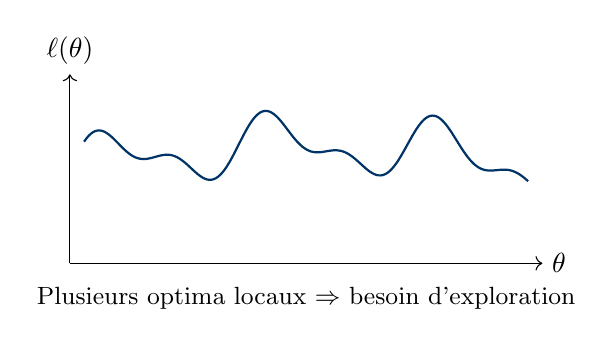
\begin{tikzpicture}[scale=0.6]
        \draw[->] (0,0) -- (10,0) node[right] {$\theta$};
        \draw[->] (0,0) -- (0,4) node[above] {$\ell(\theta)$};
        \draw[thick, darkblue, domain=0.3:9.7, samples=200] plot (\x, {0.5*sin(1.8*\x r) + 0.3*sin(3.5*\x r) - 0.02*(\x-5)^2 + 2.5});
        \node[below, font=\small] at (5,-0.3) {Plusieurs optima locaux $\Rightarrow$ besoin d'exploration};
    \end{tikzpicture}
\end{center}

\end{frame}

\begin{frame}{Recherche par grille (\textit{grid search})}

\begin{itemize}

\item \textbf{Principe :} évaluer $\ell(\theta)$ en chaque point d'une grille régulière et retenir le meilleur :
  \[
  \boxed{\hat{\theta} = \argmax_{\theta \in \mathcal{G}} \ell(\theta), \qquad \mathcal{G} = \{\theta_1, \theta_2, \ldots, \theta_M\}}
  \]

\item \textbf{Construction de la grille} (en dimension $k$) : si chaque composante prend $m$ valeurs, alors $M = m^k$ points.\newline

\item \textbf{Avantages :}
  \begin{itemize}
    \item Extrêmement simple à implémenter\newline
    \item Garantit de trouver le maximum global sur $\mathcal{G}$\newline
    \item Ne nécessite aucune dérivée\newline
  \end{itemize}

\item \textbf{Inconvénient majeur :} malédiction de la dimension ($m^k$ croît exponentiellement).

\end{itemize}

\end{frame}

\begin{frame}{Recherche par grille -- Illustration}

\begin{center}
    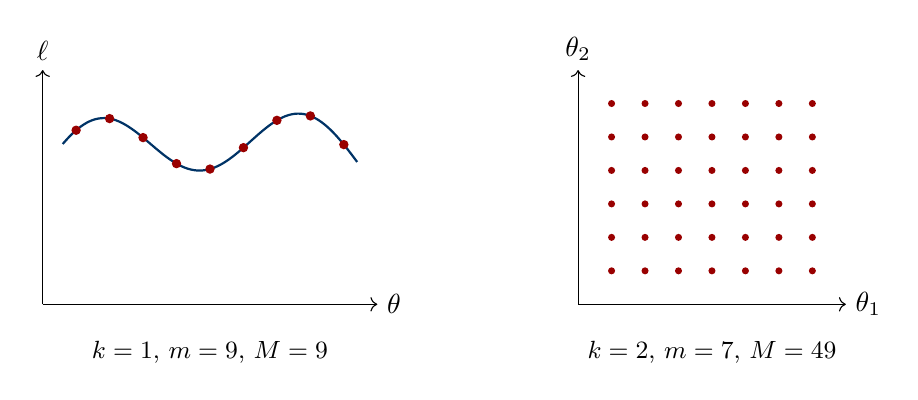
\begin{tikzpicture}[scale=0.85]
        % 1D
        \begin{scope}[shift={(-4.5,0)}]
            \draw[->] (0,0) -- (5,0) node[right] {$\theta$};
            \draw[->] (0,0) -- (0,3.5) node[above] {$\ell$};
            \draw[thick, darkblue, domain=0.3:4.7, samples=100] plot (\x, {0.5*sin(2*\x r) - 0.08*(\x-2.5)^2 + 2.5});
            % Grid points
            \foreach \x in {0.5, 1.0, ..., 4.5} {
                \pgfmathsetmacro{\yval}{0.5*sin(2*\x r) - 0.08*(\x-2.5)^2 + 2.5}
                \fill[darkred] (\x, \yval) circle (2pt);
            }
            \node[below, font=\small] at (2.5,-0.4) {$k=1$, $m=9$, $M=9$};
        \end{scope}
        % 2D
        \begin{scope}[shift={(3.5,0)}]
            \draw[->] (0,0) -- (4,0) node[right] {$\theta_1$};
            \draw[->] (0,0) -- (0,3.5) node[above] {$\theta_2$};
            \foreach \x in {0.5, 1.0, ..., 3.5} {
                \foreach \y in {0.5, 1.0, ..., 3.0} {
                    \fill[darkred] (\x, \y) circle (1.5pt);
                }
            }
            \node[below, font=\small] at (2,-0.4) {$k=2$, $m=7$, $M=49$};
        \end{scope}
    \end{tikzpicture}
\end{center}

\vspace{0.3cm}

\begin{center}
    \small
    \begin{tabular}{lccccc}
        \toprule
        Dimension $k$ & 1 & 2 & 5 & 10 & 20 \\
        \midrule
        Points ($m=10$) & 10 & 100 & $10^5$ & $10^{10}$ & $10^{20}$ \\
        \bottomrule
    \end{tabular}
\end{center}

\end{frame}

\begin{frame}{Recherche aléatoire (\textit{random search})}

\begin{itemize}

\item \textbf{Principe :} tirer $M$ points au hasard dans $\Theta$ et retenir le meilleur :
  \[
  \boxed{\hat{\theta} = \argmax_{j=1,\ldots,M} \ell(\theta_j), \qquad \theta_j \overset{i.i.d.}{\sim} \pi(\theta)}
  \]
  où $\pi$ est une distribution sur l'espace des paramètres (uniforme, normale, etc.).\newline

\item \textbf{Avantages par rapport à la grille :}
  \begin{itemize}
    \item Pas de structure rigide $\Rightarrow$ explore mieux en grande dimension\newline
    \item Coût fixe en $M$ (indépendant de $k$)\newline
    \item Si une seule composante de $\theta$ influence $\ell$, la recherche aléatoire explore $M$ valeurs de cette composante, contre $m = M^{1/k}$ pour la grille\newline
  \end{itemize}

\item \textbf{Inconvénient :} pas de garantie de couverture uniforme.

\end{itemize}

\end{frame}

\begin{frame}{Recherche aléatoire -- Grille vs aléatoire}

\begin{center}
    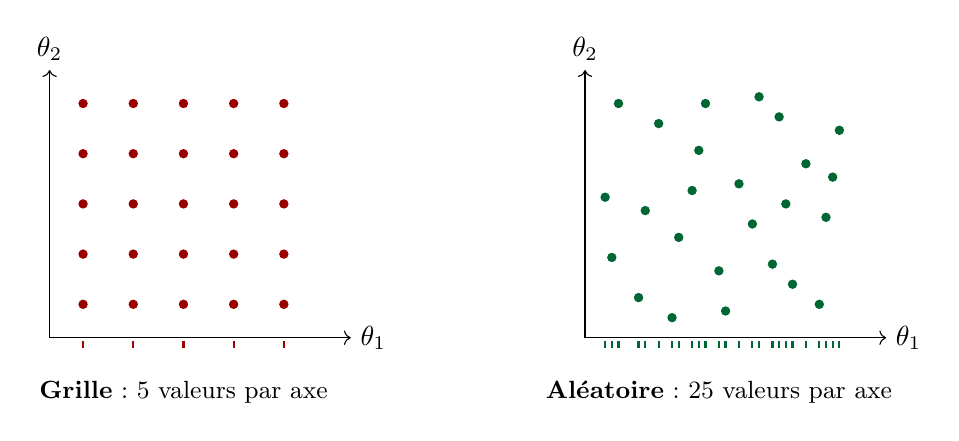
\begin{tikzpicture}[scale=0.85]
        % Grid search
        \begin{scope}[shift={(-4,0)}]
            \draw[->] (0,0) -- (4.5,0) node[right] {$\theta_1$};
            \draw[->] (0,0) -- (0,4) node[above] {$\theta_2$};
            \foreach \x in {0.5, 1.25, 2.0, 2.75, 3.5} {
                \foreach \y in {0.5, 1.25, 2.0, 2.75, 3.5} {
                    \fill[darkred] (\x, \y) circle (2pt);
                }
            }
            % Projection on axes
            \foreach \x in {0.5, 1.25, 2.0, 2.75, 3.5} {
                \draw[darkred, thick] (\x, -0.15) -- (\x, -0.05);
            }
            \node[below, font=\small] at (2,-0.5) {\textbf{Grille} : 5 valeurs par axe};
        \end{scope}
        % Random search
        \begin{scope}[shift={(4,0)}]
            \draw[->] (0,0) -- (4.5,0) node[right] {$\theta_1$};
            \draw[->] (0,0) -- (0,4) node[above] {$\theta_2$};
            % 25 random-looking points
            \foreach \pos in {(0.3,2.1),(0.8,0.6),(1.1,3.2),(1.4,1.5),(1.7,2.8),
                             (0.5,3.5),(2.1,0.4),(2.3,2.3),(2.6,3.6),(2.8,1.1),
                             (3.1,0.8),(3.3,2.6),(3.6,1.8),(3.8,3.1),(0.9,1.9),
                             (1.3,0.3),(1.8,3.5),(2.5,1.7),(3.0,2.0),(3.5,0.5),
                             (0.4,1.2),(1.6,2.2),(2.9,3.3),(3.7,2.4),(2.0,1.0)} {
                \fill[darkgreen] \pos circle (2pt);
            }
            % Projection on axes
            \foreach \x in {0.3,0.8,1.1,1.4,1.7,0.5,2.1,2.3,2.6,2.8,3.1,3.3,3.6,3.8,0.9,1.3,1.8,2.5,3.0,3.5,0.4,1.6,2.9,3.7,2.0} {
                \draw[darkgreen, thick] (\x, -0.15) -- (\x, -0.05);
            }
            \node[below, font=\small] at (2,-0.5) {\textbf{Aléatoire} : 25 valeurs par axe};
        \end{scope}
    \end{tikzpicture}
\end{center}

\vspace{0.2cm}

En projetant sur $\theta_1$, la recherche aléatoire explore \textbf{25 valeurs distinctes} contre 5 pour la grille (avec le même budget de 25 évaluations).

\end{frame}

\begin{frame}{Recherche aléatoire -- Séquences quasi-Monte Carlo}

\begin{itemize}

\item \textbf{Problème :} un tirage purement aléatoire peut laisser des «~trous~» dans l'espace de recherche.\newline

\item \textbf{Séquences à faible discrépance} (\textit{quasi-Monte Carlo}) : suites \textbf{déterministes} qui remplissent l'hypercube $[0,1]^k$ de manière plus uniforme qu'un tirage aléatoire.\newline

\item \textbf{Avantage :} pour un budget de $M$ évaluations, la couverture de l'espace est garantie. L'erreur d'approximation décroît en $O((\log M)^k / M)$ au lieu de $O(1/\sqrt{M})$.\newline

\item \textbf{Exemples classiques :} suite de Halton, suite de Sobol', hypercube latin.

\end{itemize}

\end{frame}

\begin{frame}{Séquences quasi-Monte Carlo -- Suite de Halton}

\begin{itemize}

\item \textbf{Idée :} écrire l'entier $n$ en base $b$, puis \textbf{renverser ses chiffres} après la virgule.\newline

\item \textbf{Exemple en base $b=2$ :}

\begin{center}
\small
\begin{tabular}{ccccccccc}
  \toprule
  $n$ & 1 & 2 & 3 & 4 & 5 & 6 & 7 & 8 \\
  \midrule
  Écriture binaire & 1 & 10 & 11 & 100 & 101 & 110 & 111 & 1000 \\
  Miroir & 0{,}1 & 0{,}01 & 0{,}11 & 0{,}001 & 0{,}101 & 0{,}011 & 0{,}111 & 0{,}0001 \\
  $\phi_2(n)$ & $\frac{1}{2}$ & $\frac{1}{4}$ & $\frac{3}{4}$ & $\frac{1}{8}$ & $\frac{5}{8}$ & $\frac{3}{8}$ & $\frac{7}{8}$ & $\frac{1}{16}$ \\
  \bottomrule
\end{tabular}
\end{center}

\item En dimension $k$ : on utilise une base première \textbf{différente} par dimension ($b_1=2$, $b_2=3$, $b_3=5$, \ldots). Le point $n$ est $(\phi_2(n),\, \phi_3(n),\, \phi_5(n),\, \ldots)$.

\end{itemize}

\end{frame}

\begin{frame}{Séquences quasi-Monte Carlo -- Suite de Sobol' et hypercube latin}

\begin{itemize}

\item \textbf{Suite de Sobol' :} construit des suites récurrentes \textbf{en base 2} à l'aide d'opérations binaires (XOR). Chaque dimension utilise un polynôme générateur différent sur le corps $\mathbb{F}_2 = \{0, 1\}$, ce qui garantit l'indépendance entre dimensions.\newline

\item Les polynômes générateurs sont choisis \textbf{irréductibles} sur $\mathbb{F}_2$ (analogue des nombres premiers pour les polynômes). Des tables de ces polynômes sont disponibles dans les bibliothèques standard.\newline

\item La suite de Sobol' est la plus utilisée en pratique (notamment en finance et en optimisation).\newline

\item \textbf{Hypercube latin} (\textit{Latin Hypercube Sampling}, LHS) : on découpe $[0,1]$ en $M$ strates de taille $1/M$ dans chaque dimension, et on place \textbf{exactement un point par strate}. Les strates sont appariées par une permutation aléatoire.

\end{itemize}

\end{frame}

\begin{frame}{Séquences quasi-Monte Carlo -- Illustration}

\begin{center}
    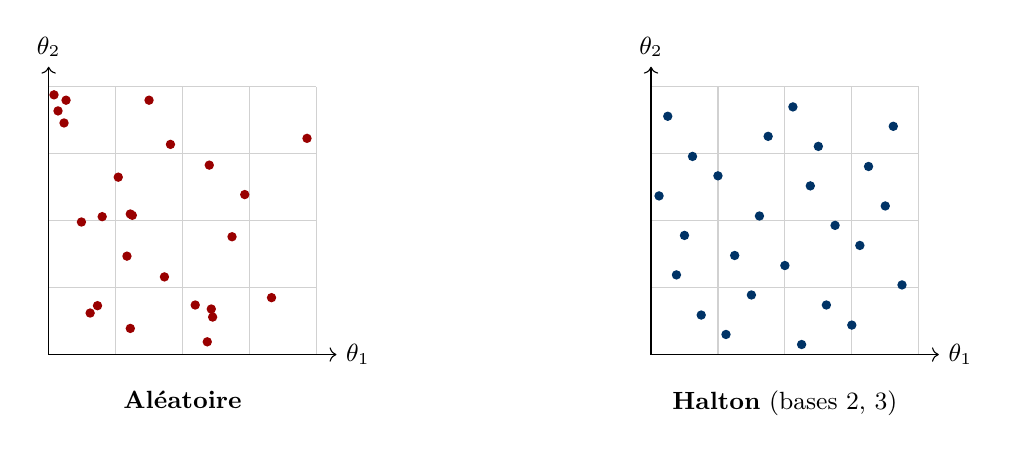
\begin{tikzpicture}[scale=0.85]
        % Random
        \begin{scope}[shift={(-4.5,0)}]
            \draw[gray!30] (0,0) grid[step=1] (4,4);
            \draw[->] (0,0) -- (4.3,0) node[right, font=\small] {$\theta_1$};
            \draw[->] (0,0) -- (0,4.3) node[above, font=\small] {$\theta_2$};
            \foreach \pos in {(1.50,3.80),(2.93,2.39),(0.62,0.62),(0.23,3.46),(2.40,2.83),
                             (0.08,3.88),(3.33,0.85),(0.73,0.73),(1.22,2.10),(1.73,1.16),
                             (2.45,0.56),(1.17,1.47),(1.82,3.14),(0.80,2.06),(2.37,0.19),
                             (2.43,0.68),(0.26,3.80),(3.86,3.23),(1.22,0.39),(2.74,1.76),
                             (0.49,1.98),(0.14,3.64),(1.04,2.65),(1.25,2.08),(2.19,0.74)} {
                \fill[darkred] \pos circle (2pt);
            }
            \node[below, font=\small] at (2,-0.4) {\textbf{Aléatoire}};
        \end{scope}
        % Halton
        \begin{scope}[shift={(4.5,0)}]
            \draw[gray!30] (0,0) grid[step=1] (4,4);
            \draw[->] (0,0) -- (4.3,0) node[right, font=\small] {$\theta_1$};
            \draw[->] (0,0) -- (0,4.3) node[above, font=\small] {$\theta_2$};
            \foreach \pos in {(2.00,1.33),(1.00,2.67),(3.00,0.44),(0.50,1.78),(2.50,3.11),
                             (1.50,0.89),(3.50,2.22),(0.25,3.56),(2.25,0.15),(1.25,1.48),
                             (3.25,2.81),(0.75,0.59),(2.75,1.93),(1.75,3.26),(3.75,1.04),
                             (0.12,2.37),(2.12,3.70),(1.12,0.30),(3.12,1.63),(0.62,2.96),
                             (2.62,0.74),(1.62,2.07),(3.62,3.41),(0.38,1.19),(2.38,2.52)} {
                \fill[darkblue] \pos circle (2pt);
            }
            \node[below, font=\small] at (2,-0.4) {\textbf{Halton} (bases 2, 3)};
        \end{scope}
    \end{tikzpicture}
\end{center}

\vspace{0.1cm}

Avec 25 points, la suite de Halton couvre l'espace de manière beaucoup plus \textbf{régulière} que le tirage aléatoire, qui laisse des zones vides et des amas.

\end{frame}

\begin{frame}{Séquences quasi-Monte Carlo -- Sobol' en 3D}

\begin{center}
    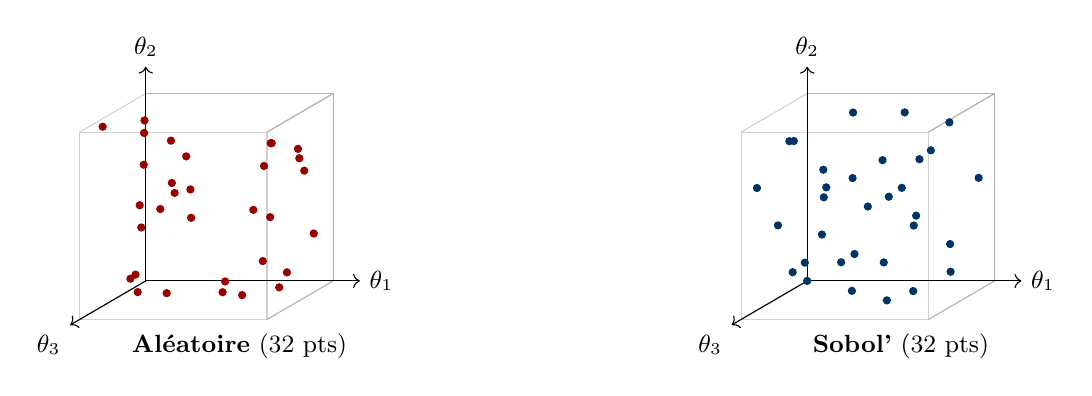
\begin{tikzpicture}
        % --- Aléatoire (gauche) ---
        \begin{scope}[shift={(-4.2cm,0cm)},
            x={(-0.24cm,-0.14cm)}, y={(0.68cm,0cm)}, z={(0cm,0.68cm)}]
            % Cube edges (back faces)
            \draw[gray!30] (3.5,0,0) -- (3.5,3.5,0) -- (3.5,3.5,3.5) -- (3.5,0,3.5) -- cycle;
            \draw[gray!30] (0,0,3.5) -- (3.5,0,3.5);
            \draw[gray!30] (0,3.5,3.5) -- (3.5,3.5,3.5);
            \draw[gray!30] (3.5,0,0) -- (0,0,0);
            % Cube edges (front faces)
            \draw[gray!50] (0,0,0) -- (0,3.5,0) -- (0,3.5,3.5) -- (0,0,3.5) -- cycle;
            \draw[gray!50] (0,3.5,0) -- (3.5,3.5,0);
            \draw[gray!50] (0,3.5,3.5) -- (3.5,3.5,3.5);
            % Axes
            \draw[->] (0,0,0) -- (0,4,0) node[right, font=\small] {$\theta_1$};
            \draw[->] (0,0,0) -- (0,0,4) node[above, font=\small] {$\theta_2$};
            \draw[->] (0,0,0) -- (4,0,0) node[below left, font=\small] {$\theta_3$};
            % Points
            \foreach \px/\py/\pz in {
                1.31/3.33/2.56,2.10/0.55/0.55,0.20/3.03/2.10,2.48/0.07/3.39,
                2.91/0.74/0.64,0.64/1.06/1.84,1.51/1.02/2.14,0.49/1.02/1.28,
                1.60/2.75/0.70,1.80/2.07/0.16,2.13/0.60/0.23,3.32/3.38/2.83,
                1.07/0.34/2.39,1.54/0.43/1.73,0.12/3.18/0.91,2.32/1.09/1.82,
                1.91/0.65/3.39,2.71/3.29/3.13,2.09/3.23/0.31,0.69/0.16/1.14,
                1.36/0.95/2.90,1.25/0.98/1.90,0.49/2.81/0.26,3.45/2.70/0.70,
                0.02/2.85/2.47,2.55/2.70/0.26,1.25/0.41/3.02,2.18/1.16/0.22,
                1.09/1.14/2.55,2.23/3.11/1.65,0.42/2.50/2.66,1.96/2.70/1.73} {
                \fill[darkred] (\px,\py,\pz) circle (1.5pt);
            }
            \node[below, font=\small] at (0,1.75,-0.8) {\textbf{Aléatoire} (32 pts)};
        \end{scope}
        % --- Sobol' (droite) ---
        \begin{scope}[shift={(4.2cm,0cm)},
            x={(-0.24cm,-0.14cm)}, y={(0.68cm,0cm)}, z={(0cm,0.68cm)}]
            % Cube edges (back faces)
            \draw[gray!30] (3.5,0,0) -- (3.5,3.5,0) -- (3.5,3.5,3.5) -- (3.5,0,3.5) -- cycle;
            \draw[gray!30] (0,0,3.5) -- (3.5,0,3.5);
            \draw[gray!30] (0,3.5,3.5) -- (3.5,3.5,3.5);
            \draw[gray!30] (3.5,0,0) -- (0,0,0);
            % Cube edges (front faces)
            \draw[gray!50] (0,0,0) -- (0,3.5,0) -- (0,3.5,3.5) -- (0,0,3.5) -- cycle;
            \draw[gray!50] (0,3.5,0) -- (3.5,3.5,0);
            \draw[gray!50] (0,3.5,3.5) -- (3.5,3.5,3.5);
            % Axes
            \draw[->] (0,0,0) -- (0,4,0) node[right, font=\small] {$\theta_1$};
            \draw[->] (0,0,0) -- (0,0,4) node[above, font=\small] {$\theta_2$};
            \draw[->] (0,0,0) -- (4,0,0) node[below left, font=\small] {$\theta_3$};
            % Points
            \foreach \px/\py/\pz in {
                0.00/0.00/0.00,1.75/1.75/1.75,2.62/0.88/0.88,0.88/2.62/2.62,
                1.31/1.31/2.19,3.06/3.06/0.44,2.19/0.44/3.06,0.44/2.19/1.31,
                0.66/1.09/3.28,2.41/2.84/1.53,3.28/0.22/2.41,1.53/1.97/0.66,
                1.09/0.66/1.09,2.84/2.41/2.84,1.97/1.53/0.22,0.22/3.28/1.97,
                0.33/1.64/1.64,2.08/3.39/3.39,2.95/0.77/0.77,1.20/2.52/2.52,
                1.64/0.33/2.95,3.39/2.08/1.20,2.52/1.20/2.08,0.77/2.95/0.33,
                0.55/0.55/1.86,2.30/2.30/0.11,3.17/1.42/2.73,1.42/3.17/0.98,
                0.98/0.98/0.55,2.73/2.73/2.30,1.86/0.11/1.42,0.11/1.86/3.17} {
                \fill[darkblue] (\px,\py,\pz) circle (1.5pt);
            }
            \node[below, font=\small] at (0,1.75,-0.8) {\textbf{Sobol'} (32 pts)};
        \end{scope}
    \end{tikzpicture}
\end{center}

\vspace{0.1cm}

En dimension 3, la suite de Sobol' remplit le cube $[0,1]^3$ de manière \textbf{quasi uniforme}, tandis que le tirage aléatoire produit des amas et des vides.

\end{frame}

\begin{frame}{Recuit simulé (\textit{simulated annealing}) -- Principe}

\begin{itemize}

\item \textbf{Analogie physique :} en métallurgie, un refroidissement lent permet aux atomes de trouver une configuration d'énergie minimale (cristal). Un refroidissement rapide fige les défauts (verre).\newline

\item \textbf{Idée :} accepter parfois des solutions \textbf{moins bonnes} pour échapper aux optima locaux. La probabilité d'accepter une dégradation \textbf{décroît} au fil du temps.\newline

\item \textbf{Paramètre clé :} la \textbf{température} $T$, qui contrôle l'exploration :
  \begin{itemize}
    \item $T$ élevé $\Rightarrow$ forte exploration (on accepte souvent des dégradations)\newline
    \item $T$ faible $\Rightarrow$ exploitation locale (comportement glouton)\newline
  \end{itemize}

\item $T$ décroît selon un \textbf{schéma de refroidissement} : $T_0 > T_1 > T_2 > \cdots > 0$

\end{itemize}

\end{frame}

\begin{frame}{Recuit simulé -- Algorithme}

\begin{itemize}

\item À chaque itération $p$ :

  \begin{enumerate}
    \item Tirer un candidat $\theta' = \theta_{(p)} + \varepsilon$, \quad $\varepsilon \sim \mathcal{N}(0, \sigma^2 I)$\newline
    \item Calculer $\Delta = \ell(\theta') - \ell(\theta_{(p)})$\newline
    \item \textbf{Règle d'acceptation de Metropolis :}
  \end{enumerate}

  \[
  \boxed{\theta_{(p+1)} = \begin{cases}
      \theta' & \text{si } \Delta \geq 0 \quad \text{(amélioration : toujours acceptée)} \\
      \theta' & \text{avec probabilité } e^{\Delta / T_p} \quad \text{si } \Delta < 0 \\
      \theta_{(p)} & \text{sinon}
  \end{cases}}
  \]

\item La probabilité d'accepter une dégradation $\Delta < 0$ est $e^{\Delta/T_p}$ :
  \begin{itemize}
    \item $T_p$ grand : $e^{\Delta/T_p} \approx 1$ (on accepte presque tout)\newline
    \item $T_p$ petit : $e^{\Delta/T_p} \approx 0$ (on n'accepte que les améliorations)
  \end{itemize}

\end{itemize}

\end{frame}

\begin{frame}{Recuit simulé -- Schémas de refroidissement}

\begin{itemize}

\item Schémas classiques :
  \begin{itemize}
    \item \textbf{Géométrique :} $T_p = \alpha^p T_0$, \quad $\alpha \in (0.9, \, 0.99)$\newline
    \item \textbf{Logarithmique :} $T_p = \dfrac{T_0}{\ln(1+p)}$ \quad (convergence théorique garantie)\newline
    \item \textbf{Linéaire :} $T_p = T_0\left(1 - \dfrac{p}{P}\right)$, \quad $P$ = nombre total d'itérations\newline
  \end{itemize}

\item En pratique, le schéma géométrique avec $\alpha \approx 0.95$ est le plus utilisé.

\end{itemize}

\vspace{0.2cm}

\begin{center}
    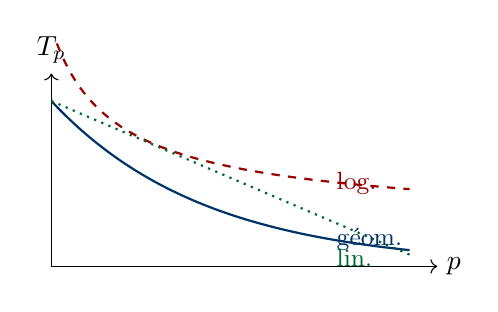
\begin{tikzpicture}[scale=0.7]
        \draw[->] (0,0) -- (7,0) node[right] {$p$};
        \draw[->] (0,0) -- (0,3.5) node[above] {$T_p$};
        \draw[thick, darkblue, domain=0:6.5, samples=100] plot (\x, {3*0.7^\x});
        \draw[thick, darkred, dashed, domain=0.1:6.5, samples=100] plot (\x, {3/ln(1+\x+1)});
        \draw[thick, darkgreen, dotted, domain=0:6.5, samples=100] plot (\x, {3*(1-\x/7)});
        \node[right, darkblue, font=\small] at (5,0.5) {géom.};
        \node[right, darkred, font=\small] at (5,1.5) {log.};
        \node[right, darkgreen, font=\small] at (5,0.15) {lin.};
    \end{tikzpicture}
\end{center}

\end{frame}

\begin{frame}{Recuit simulé -- Illustration}

\begin{center}
    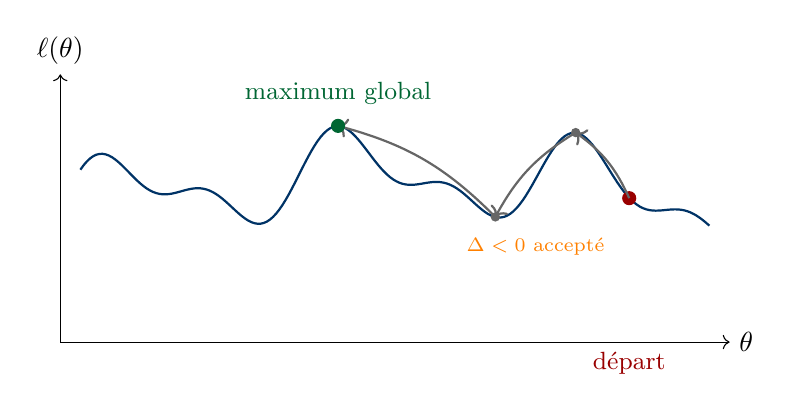
\begin{tikzpicture}[scale=0.85]
        \draw[->] (0,0) -- (10,0) node[right] {$\theta$};
        \draw[->] (0,0) -- (0,4) node[above] {$\ell(\theta)$};
        \draw[thick, darkblue, domain=0.3:9.7, samples=200] plot (\x, {0.5*sin(1.8*\x r) + 0.3*sin(3.5*\x r) - 0.02*(\x-5)^2 + 2.5});
        % Trajectory
        \fill[darkred] (8.5,2.15) circle (3pt);
        \node[below, darkred, font=\small] at (8.5,0) {départ};
        \draw[->, thick, gray] (8.5,2.15) to[bend right=15] (7.7,3.13);
        \fill[gray] (7.7,3.13) circle (2pt);
        \draw[->, thick, gray] (7.7,3.13) to[bend right=15] (6.5,1.87);
        \fill[gray] (6.5,1.87) circle (2pt);
        \node[below, orange, font=\scriptsize] at (7.1,1.7) {$\Delta < 0$ accepté};
        \draw[->, thick, gray] (6.5,1.87) to[bend right=15] (4.15,3.23);
        \fill[darkgreen] (4.15,3.23) circle (3pt);
        \node[above, darkgreen, font=\small] at (4.15,3.4) {maximum global};
    \end{tikzpicture}
\end{center}

\vspace{0.2cm}

L'acceptation occasionnelle de dégradations permet de \textbf{franchir les vallées} entre optima locaux et d'atteindre le maximum global.

\end{frame}

\begin{frame}{Essaim de particules (\textit{particle swarm optimization})}

\begin{itemize}

\item \textbf{Analogie :} comportement collectif d'un banc de poissons ou d'une volée d'oiseaux. Chaque individu ajuste sa trajectoire en fonction de sa propre expérience et de celle du groupe.\newline

\item \textbf{Population :} $N_p$ particules, chacune ayant une position $\theta_i$ et une vitesse $v_i$.\newline

\item \textbf{Mémoires :}
  \begin{itemize}
    \item $\theta_i^*$ : meilleure position visitée par la particule $i$ (\textit{personal best})\newline
    \item $\theta_g^*$ : meilleure position trouvée par l'essaim entier (\textit{global best})\newline
  \end{itemize}

\item \textbf{Initialisation :} les positions $\theta_i$ sont tirées aléatoirement dans l'espace de recherche. Les vitesses initiales $v_i$ sont tirées dans $\left[-\frac{\theta_{\max} - \theta_{\min}}{2}, \frac{\theta_{\max} - \theta_{\min}}{2}\right]$ (ou mises à zéro).

\end{itemize}

\end{frame}

\begin{frame}{Essaim de particules -- Mise à jour}

\begin{itemize}

\item \textbf{Vitesse :} la vitesse $v_i$ détermine la direction et l'amplitude du déplacement de chaque particule. Elle combine trois composantes :
  \begin{itemize}
    \item \textbf{Inertie} ($\omega v_i$) : tendance à continuer dans la même direction\newline
    \item \textbf{Cognitive} ($c_1 r_1 (\theta_i^* - \theta_i)$) : attraction vers le meilleur point personnel\newline
    \item \textbf{Sociale} ($c_2 r_2 (\theta_g^* - \theta_i)$) : attraction vers le meilleur point du groupe\newline
  \end{itemize}

\item \textbf{Règle de mise à jour :}
  \[
  \boxed{v_i \leftarrow \omega v_i + c_1 r_1 (\theta_i^* - \theta_i) + c_2 r_2 (\theta_g^* - \theta_i)}
  \]
  \[
  \theta_i \leftarrow \theta_i + v_i
  \]
  où $r_1, r_2 \sim \mathcal{U}(0,1)$ sont retirés à chaque itération et pour chaque particule.

\end{itemize}

\end{frame}

\begin{frame}{Essaim de particules -- Paramètres et propriétés}

\begin{itemize}

\item \textbf{Paramètres :}
  \begin{itemize}
    \item $\omega \in (0, 1)$ : inertie (mémoire de la direction précédente)\newline
    \item $c_1$ : attraction vers le \textit{personal best} (composante cognitive)\newline
    \item $c_2$ : attraction vers le \textit{global best} (composante sociale)\newline
    \item $r_1, r_2 \sim \mathcal{U}(0,1)$ : aléa à chaque itération\newline
  \end{itemize}

\item Valeurs classiques : $\omega = 0.7$, $c_1 = c_2 = 1.5$, $N_p = 20$--$50$.\newline

\item \textbf{Avantages :}
  \begin{itemize}
    \item Ne nécessite aucune dérivée\newline
    \item Parallélisable (évaluations indépendantes)\newline
    \item Efficace en dimension modérée
  \end{itemize}

\end{itemize}

\end{frame}

\begin{frame}{Essaim de particules -- Illustration}

\begin{center}
    \begin{tikzpicture}[scale=0.85]
        \draw[->] (0,0) -- (9,0) node[right] {$\theta_1$};
        \draw[->] (0,0) -- (0,6) node[above] {$\theta_2$};
        % Global best
        \fill[darkgreen] (6,4) circle (4pt);
        \node[above right, darkgreen, font=\small] at (6,4) {$\theta_g^*$};
        % Particles with velocities
        \fill[darkblue] (2,1.5) circle (3pt);
        \draw[->, thick, darkblue] (2,1.5) -- (2.8,2.3);
        \fill[darkblue] (3,4.5) circle (3pt);
        \draw[->, thick, darkblue] (3,4.5) -- (3.9,4.4);
        \fill[darkblue] (5,2) circle (3pt);
        \draw[->, thick, darkblue] (5,2) -- (5.6,2.8);
        \fill[darkblue] (7,1.5) circle (3pt);
        \draw[->, thick, darkblue] (7,1.5) -- (6.8,2.4);
        \fill[darkblue] (1.5,4) circle (3pt);
        \draw[->, thick, darkblue] (1.5,4) -- (2.4,4.1);
        \fill[darkblue] (4,3) circle (3pt);
        \draw[->, thick, darkblue] (4,3) -- (4.7,3.4);
        \fill[darkblue] (7.5,4.5) circle (3pt);
        \draw[->, thick, darkblue] (7.5,4.5) -- (7.1,4.4);
        % Dashed lines to global best
        \draw[dashed, gray, thin] (2,1.5) -- (6,4);
        \draw[dashed, gray, thin] (5,2) -- (6,4);
        \draw[dashed, gray, thin] (4,3) -- (6,4);
    \end{tikzpicture}
\end{center}

\vspace{0.2cm}

Chaque particule ({\color{darkblue}$\bullet$}) est attirée vers le meilleur global ({\color{darkgreen}$\bullet$}) tout en gardant une part d'inertie et d'exploration individuelle.

\end{frame}

\begin{frame}{Méthodes globales -- Récapitulatif}

\begin{center}
    \small
    \renewcommand{\arraystretch}{1.3}
    \begin{tabular}{lccc}
        \toprule
        \textbf{Méthode} & \textbf{Dérivées} & \textbf{Scalabilité} & \textbf{Garantie globale} \\
        \midrule
        Grille & Non & Très faible & Sur $\mathcal{G}$ \\
        Aléatoire & Non & Faible & Asymptotique \\
        Recuit simulé & Non & Moyenne & Théorique (log.) \\
        Essaim de particules & Non & Moyenne & Non \\
        \bottomrule
    \end{tabular}
\end{center}

\vspace{0.3cm}

\begin{itemize}

\item Aucune de ces méthodes ne nécessite de dérivées.\newline

\item En pratique, on les utilise pour \textbf{trouver un bon point de départ} $\theta_{(0)}$, puis on affine avec une méthode de gradient (Newton-Raphson, BHHH, etc.).\newline

\item Le recuit simulé est le plus utilisé en économétrie pour les fonctions non concaves.

\end{itemize}

\end{frame}

%==============================================================================
\section{Méthodologie de programmation}
%==============================================================================

\begin{frame}{Méthodologie -- Vérifier la fonction objectif}

\begin{itemize}

\item \textbf{Méthodes :}
  \begin{itemize}
    \item Calcul analytique : dériver $\ell(\theta)$ à la main\newline
    \item Vérification croisée : comparer avec les références (articles, manuels)\newline
    \item Cas particuliers : tester sur des exemples simples à solution connue\newline
  \end{itemize}

\item \textbf{Erreurs courantes :}
  \begin{itemize}
    \item Oubli du signe moins devant certains termes\newline
    \item Erreurs dans les constantes (facteur $\frac{1}{2}$, $\frac{N}{2}$, etc.)\newline
    \item Confusion entre $\ln f$ et $f$
  \end{itemize}

\end{itemize}

\end{frame}

\begin{frame}{Méthodologie -- Vérifier le gradient}

\begin{itemize}

\item Comparer le gradient analytique $s(\theta)$ avec l'approximation numérique :
  \[
  s_j^{\text{num}}(\theta) \approx \frac{\ell(\theta + h e_j) - \ell(\theta - h e_j)}{2h}
  \]
  où $e_j$ est le $j$-ème vecteur de base et $h \approx 10^{-5}$.\newline

\item Critère de vérification :
  \[
  \frac{|s_j^{\text{ana}} - s_j^{\text{num}}|}{|s_j^{\text{ana}}| + |s_j^{\text{num}}| + \varepsilon} < \text{tol}
  \]
  avec $\text{tol} \approx 10^{-4}$ à $10^{-6}$.\newline

\item Cette étape permet de détecter les erreurs dans $\ell$ et dans $s$.

\end{itemize}

\end{frame}

\begin{frame}{Méthodologie -- Vérifier le hessien}

\begin{itemize}

\item Calculer le hessien numériquement \textbf{à partir du gradient analytique} :
  \[
  H_{jk}^{\text{num}}(\theta) \approx \frac{s_j(\theta + h e_k) - s_j(\theta - h e_k)}{2h}
  \]

\item Calculer $H$ numériquement à partir de $\ell$ (différences finies d'ordre 2) cumule les erreurs d'approximation $\Rightarrow$ utiliser le gradient analytique vérifié comme base.\newline

\item On peut conserver les dérivées numériques si le calcul analytique est trop complexe.

\end{itemize}

\end{frame}

\begin{frame}{Méthodologie -- Paramétrer le programme}

\begin{itemize}

\item \textbf{Objectif :} Éviter toute intervention manuelle après vérification $\Rightarrow$ source d'erreurs.\newline

\item \textbf{Bonnes pratiques :}
  \begin{itemize}
    \item Utiliser des paramètres pour les tolérances, $\lambda$, $\alpha$\newline
    \item Créer des fonctions réutilisables (log-vraisemblance, gradient, hessien)\newline
    \item Documenter le code\newline
    \item Prévoir des messages d'erreur informatifs\newline
    \item Sauvegarder les résultats intermédiaires
  \end{itemize}

\end{itemize}

\end{frame}

\begin{frame}{Méthodologie -- Checklist}

\begin{center}
    \small
    \renewcommand{\arraystretch}{1.3}
    \begin{tabular}{ll}
        \toprule
        \textbf{Élément} & \textbf{Vérification} \\
        \midrule
        Log-vraisemblance $\ell$ & $\square$ Formule correcte \\
        & $\square$ Cas particuliers testés \\
        \midrule
        Gradient $s$ & $\square$ Dérivation analytique \\
        & $\square$ Vérification numérique \\
        \midrule
        Hessien $H$ & $\square$ Dérivation analytique \\
        & $\square$ Vérification numérique \\
        & $\square$ Définie négative à l'optimum \\
        \midrule
        Convergence & $\square$ Critères d'arrêt atteints \\
        & $\square$ Résultats stables (différents $\theta_{(0)}$) \\
        \bottomrule
    \end{tabular}
\end{center}

\end{frame}

%==============================================================================
\section{Récapitulatif}
%==============================================================================

\begin{frame}{Récapitulatif -- Synthèse}

\begin{center}
    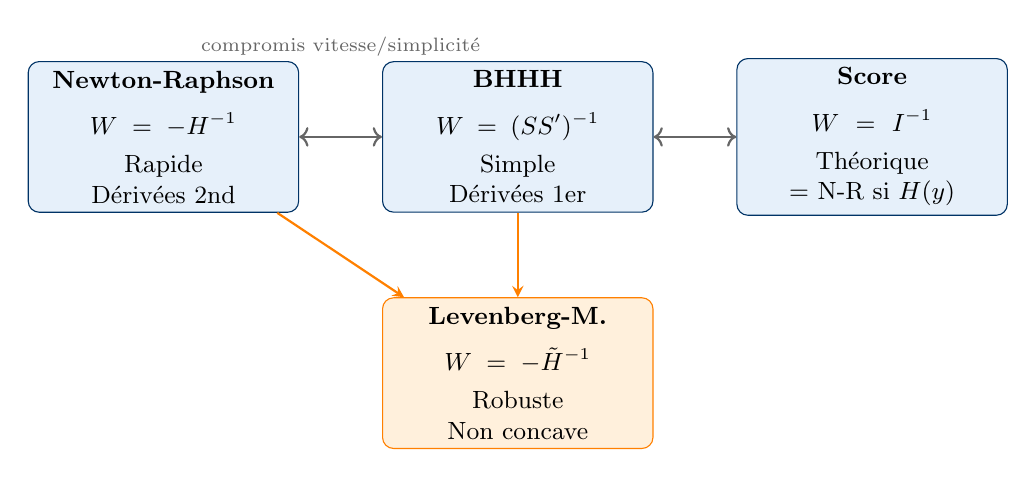
\begin{tikzpicture}[
        node distance=0.8cm,
        box/.style={rectangle, draw=darkblue, fill=lightblue, text width=3.2cm, align=center, minimum height=1.8cm, rounded corners, font=\small},
        arrow/.style={->, >=stealth, thick, darkblue}
    ]
    \node[box] (nr) at (0,0) {\textbf{Newton-Raphson}\\[0.2cm]$W = -H^{-1}$\\[0.1cm]Rapide\\Dérivées 2nd};
    \node[box] (bhhh) at (4.5,0) {\textbf{BHHH}\\[0.2cm]$W = (SS')^{-1}$\\[0.1cm]Simple\\Dérivées 1er};
    \node[box] (score) at (9,0) {\textbf{Score}\\[0.2cm]$W = I^{-1}$\\[0.1cm]Théorique\\$= $ N-R si $H(y)$};
    \node[box, fill=lightorange, draw=orange] (lm) at (4.5,-3) {\textbf{Levenberg-M.}\\[0.2cm]$W = -\tilde{H}^{-1}$\\[0.1cm]Robuste\\Non concave};
    \draw[<->, thick, gray] (nr) -- (bhhh);
    \draw[<->, thick, gray] (bhhh) -- (score);
    \draw[arrow, orange] (nr) -- (lm);
    \draw[arrow, orange] (bhhh) -- (lm);
    \node[above, font=\scriptsize, gray] at (2.25,0.9) {compromis vitesse/simplicité};
    \end{tikzpicture}
\end{center}

\end{frame}

\begin{frame}{Récapitulatif -- Formules essentielles}

\begin{itemize}

\item Forme générale :
  \[
  \boxed{\theta_{(p+1)} = \theta_{(p)} + \lambda W_{(p)} s(\theta_{(p)})}
  \]

\end{itemize}

\vspace{0.2cm}

\begin{center}
    \renewcommand{\arraystretch}{1.5}
    \begin{tabular}{ll}
        \toprule
        \textbf{Algorithme} & \textbf{Matrice $W_{(p)}$} \\
        \midrule
        Newton-Raphson & $-H(\theta_{(p)})^{-1}$ \\
        BHHH & $\left(\sum_i s_i s_i'\right)^{-1}$ \\
        Score & $\left(\sum_i \mathbb{E}[s_i s_i']\right)^{-1}$ \\
        Levenberg-Marquardt & $-\left(H - (1+\alpha)\mu_H I\right)^{-1}$ \\
        \bottomrule
    \end{tabular}
\end{center}

\end{frame}

\begin{frame}{Récapitulatif -- Points clés}

\begin{enumerate}

\item \textbf{Concavité :} si $\ell$ est concave, tout algorithme croissant converge.\newline

\item \textbf{Newton-Raphson :} rapide mais nécessite $H$.\newline

\item \textbf{BHHH :} simple, utilise seulement le gradient.\newline

\item \textbf{Levenberg-Marquardt :} robuste pour les cas non concaves.\newline

\item \textbf{Vérification :} toujours contrôler numériquement les dérivées.\newline

\item \textbf{CSO :} vérifier que $H(\hat{\theta}_N) \prec 0$ à la fin.

\end{enumerate}

\end{frame}

\begin{frame}{Références}

\begin{itemize}

\item Gouriéroux, C. et Monfort, A. (1989). \textit{Statistique et Modèles Économétriques}, Economica, ch. XIII\newline

\item Davidson, R. et MacKinnon, J. (2004). \textit{Econometric Theory and Methods}, Oxford\newline

\item Greene, W. (2018). \textit{Econometric Analysis}, 8th ed., Pearson\newline

\item Berndt, E., Hall, B., Hall, R. et Hausman, J. (1974). ``Estimation and Inference in Nonlinear Structural Models'', \textit{Annals of Economic and Social Measurement}, 3(4), 653-665.

\end{itemize}

\end{frame}

\end{document}
